\chapter{序論}
\label{chap:intro}

本章では,本研究の研究背景と研究目的について説明する.
\secref{sec:background}で研究背景,
\secref{sec:purpose}で研究目的,
\secref{sec:structure}で本論文の構成について述べる.

\section{研究背景}\label{sec:background}
\indent
音楽演奏を題材としたアニメーションは多く存在する.
テレビで放映されたアニメーションの例を挙げると,『のだめカンタービレ』,『けいおん!』,『響け!ユーフォニアム』が相当する.
これらのアニメーションは,セル画であったり3DCGであったり,製作方法はさまざまであるが,いずれも実際に演奏する演奏者の身体の動きに近い演奏アニメーションが生成されている.
楽器の輝きや形状なども忠実に再現されている.
しかし,楽器を演奏するキャラクタの運指や身体の動きが,音楽に完全に同期されていないことがある.
特に速いフレーズや,複雑なリズムを演奏するシーンで,このようなアーティファクトが起きやすい.
また,表情からも不自然さを感じることがある.
実際にアンケートをとったところ,楽器経験者を中心に,演奏アニメーションが不自然であると感じている者が多くいることが分かった.\figref{fig:q1}は,その集計結果である.
\begin{figure}[h]
	\centering
	\subcaptionbox{\textgt{吹奏楽・オーケストラ団体への所属経験者または金管楽器経験者の回答}
		\label{fig:ans1_1}}{
		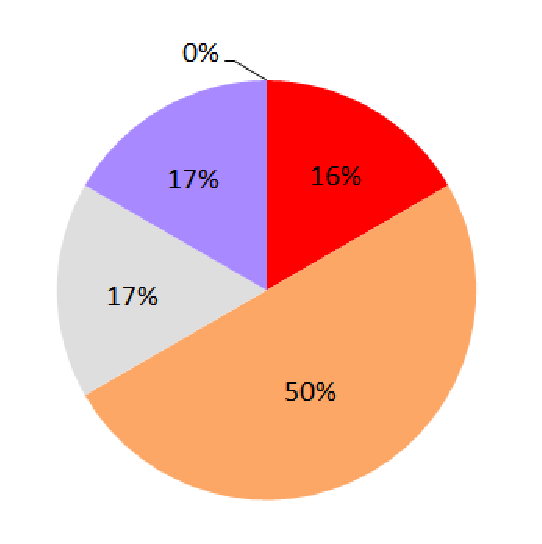
\includegraphics[width=4.8cm]{fig/chap1/ans1-1.eps}}
	\subcaptionbox{\textgt{(a)にはあてはまらない楽器経験者の回答}
		\label{fig:ans1_2}}{
		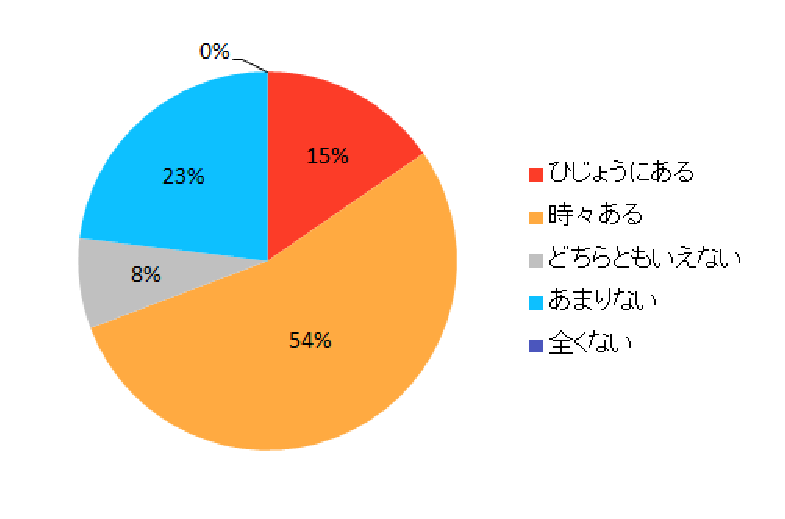
\includegraphics[width=4.8cm]{fig/chap1/ans1-2.eps}}
	\subcaptionbox{\textgt{楽器未経験者の回答}
		\label{fig:ans1_3}}{
		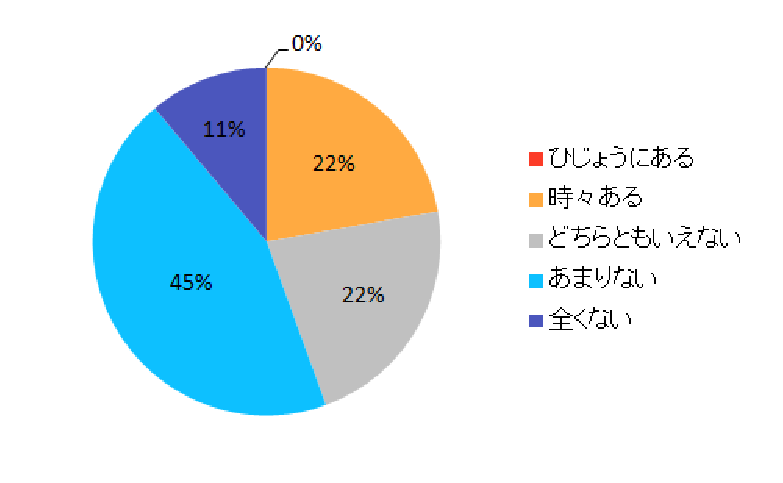
\includegraphics[width=4.8cm]{fig/chap1/ans1-3.eps}}
	\caption{演奏アニメーションが不自然であると感じることがあるかどうか}
	\label{fig:q1}
\end{figure}
\par
演奏アニメーションが不自然であると感じる点は,指使いが間違っている点,指や身体の動きがリズムに合っていない点,演奏している雰囲気が感じられない点,表情など,吹奏楽やオーケストラ団体への所属経験や楽器の経験に関わらず,さまざまであるという結果も得た.\\
\indent
これらの不自然さを解消するためには,身体の動きを1つずつ音階やリズムなどに手動で合わせる必要がある.
しかし,この方法はひじょうに効率が悪く,多くの時間と労力が必要となる.

\section{研究目的}\label{sec:purpose}
\secref{sec:background}で述べた課題を解消するため,本研究では,管楽器を演奏するキャラクタの吹奏アニメーションを,音源から自動的に生成することを目指す.
より具体的には,実際の演奏アニメーション制作フローに沿わせるため,楽曲は電子楽器を用いてMIDI(Musical Instrument Digital Interface)音源として生成する.
次に,作成した楽曲を解析することにより,吹奏の情報を得る.
最後に,得られた情報をキャラクタの身体の動きや表情,そして管楽器に適用することにより,音源に同期した自然な吹奏アニメーションを実現する.
提案手法の対象ユーザはアニメータとし,最終的にはアニメータの作業支援を目的とする.
また,本研究は,同研究室学士4年の武内航と共同で進めてきた.
武内が担当した部分については,その旨を明記する.

\section{本論文の構成}\label{sec:structure}
本論文は次章以降,以下のように構成される.
\begin{description}
	\setlength{\itemindent}{4pt}
	%\setlength{\itemsep}{-4pt}
	%\setlength{\labelwidth}{5zw}
	\item[第2章 関連研究] \mbox{}\\
	\hspace{3ex}アニメーションや音を自動生成する研究や,吹奏楽に関連した研究を紹介する.
	\item[第3章 提案手法] \mbox{}\\
	\hspace{3ex} \ref{sec:purpose}節で示した研究目的を達成するための手法を説明する.
	\item[第4章 自動生成結果と評価] \mbox{}\\
	\hspace{3ex} アニメーションの自動生成結果について述べ,この結果に対する評価をまとめる.
	\item[第5章 結論] \mbox{}\\
	\hspace{3ex} 本研究の結論を述べ,今後の課題に言及する.
\end{description}
\indent
なお,本研究の成果はVisual Computing/グラフィクスとCAD合同シンポジウム2017においてポスター\cite{vc}として発表した.そして,映像表現・芸術科学フォーラム2018(2018年3月)において発表し,Cyberworlds(2018年8月)に論文投稿する予定である.